\begin{figure}[ht] 
 	\centering 
 	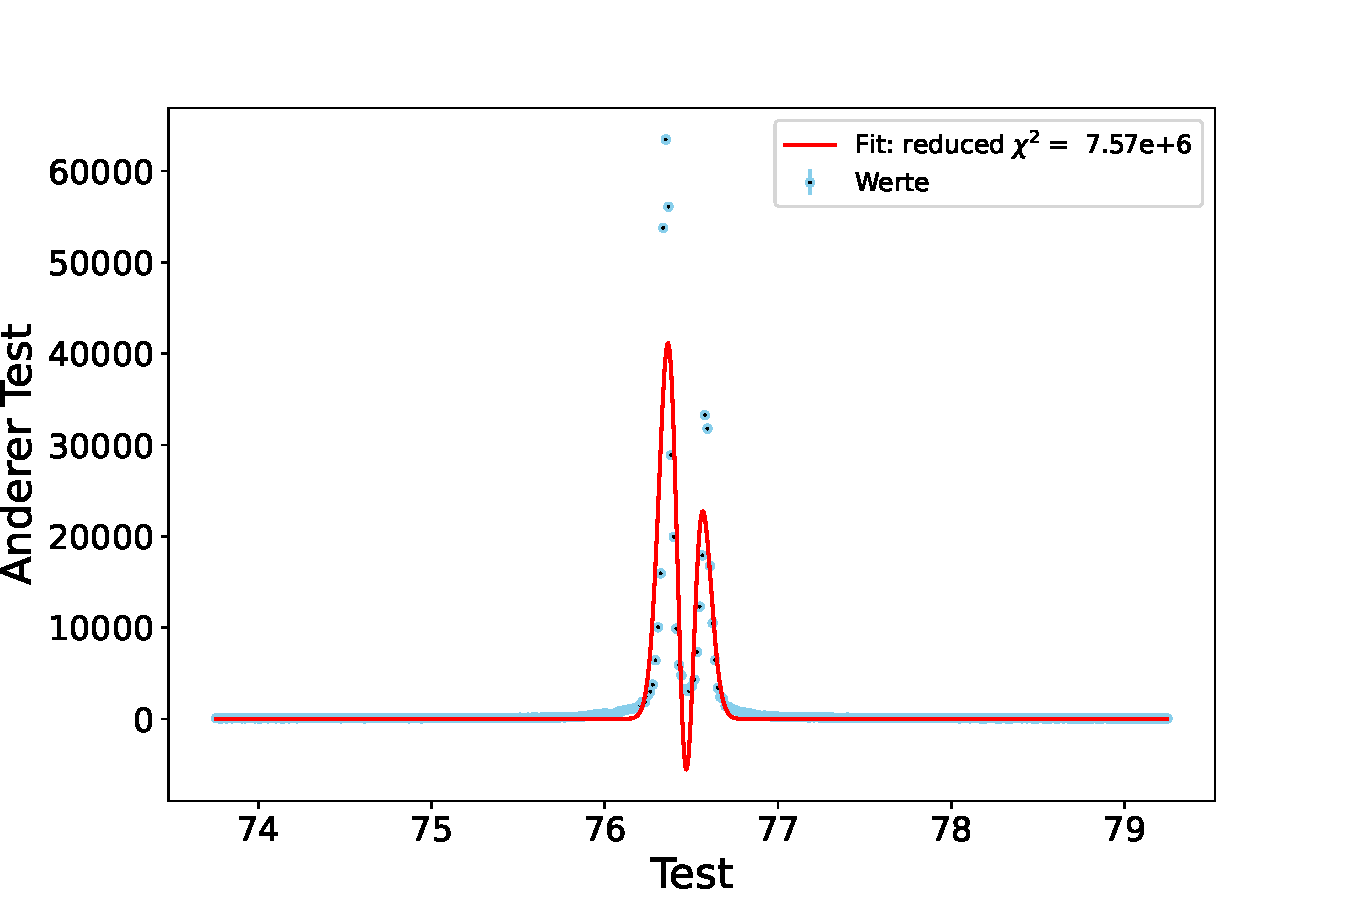
\includegraphics[width= 0.65 \textwidth]{Fits/data_test_Fit.pdf} 
	\caption{data_test, Fit} 
 	\label{fig:data_test, Fit} 
\end{figure}
 \\ 
\begin{table}[ht] 
\centering 
\caption{my-table} 
\label{tab:my-table}
\begin{tabular}{|l|c|}
\hline
Parameter Name	&	Wert \\ \hline
aamplitude	&	 4791547.135 \pm  110728642176.891\\ \hline
acenter	&	 76.458 \pm  0.515\\ \hline
asigma	&	 0.069 \pm  1.303\\ \hline
bamplitude	&	-4784466.3879 \pm  110728642255.905\\ \hline
bcenter	&	 76.458 \pm  0.541\\ \hline
bsigma	&	 0.0689 \pm  1.302\\ \hline
afwhm	&	 0.162 \pm  3.069\\ \hline
aheight	&	 27701434.746 \pm  640680127018.875\\ \hline
bfwhm	&	 0.162 \pm  3.067\\ \hline
bheight	&	-27705246.7021 \pm  640668841582.680\\ \hline
\end{tabular} 
\end{table}